\section{teaching}

Inmaculada Garcia Fernandez
\section {2.A. Does your university run joint degrees (e.g. X and Informatics, Informatics and X, X with Informatics, Informatics with X). If yes, what are they?}

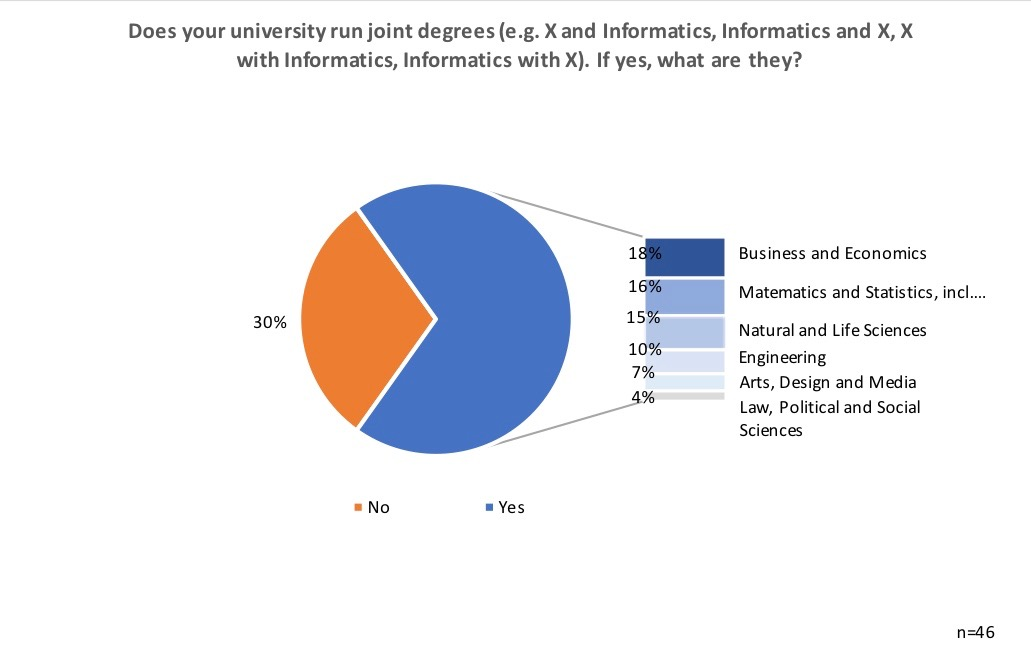
\includegraphics[width = \linewidth]{charts/2a.jpg}

Only 30\% of the universities does not run a joint degree including Informatics.Within this group of universities, some of them specify that all their programs entails to some extend technical aspects of IT, like programming or data base technology or there are some joint programmes, e.g. a Data Science BSc programme that joins CS, Math and Industrial Engineering, and an MSc major in Game Design and Production jointly with the Arts School, but these are collaborative initiatives in new directions, where the CS Department is one of the partners; the Business School has their own small Informatics programme.

The remaing 70\% of the universities run some joint degrees, the most popular joint degrees including Informatics are  Business and Economics (Business Informatics; CS and Business; Computing and Economics; Information systems combining Informatics and Business Administration; CS and Management; Informatics and Economics; Informatics and Finance; Economics and Business Informatics; Data Science and Entrepreneurship) followed by Mathematics and Statistics (Informatics and Mathematics; Data Science; Informatics and Applied Mathematics; Informatics and Statistics), Natural and Life Sciences (Bioinformatics; Informatics and Natural Sciences; CS and Physics; AI for Biomedicine; Precision Medicine; Geoinformatics; Chemistry and Informatics; Biology and Informatics; Informatics Health) and Engineering (Computational Engineering; Computer Engineering; Electronics and Information Engineering; Informatics and Electronics; Informatics and Telecommunications; Informatics and Cybernetics; Informatics and Mechatronics; Informatics and Aerospace Engineering; Informatics and Civil Engineering; Informatics and Industrial Engineering). Joint degrees in informatics plus Arts, Design and Media (Technical Communication; Design Informatics; CS and communication, CS and design; ICT and media; Informatics and information science; Informatics and library science) or Law, Political and Social Sciences (Law and Informatics; Social sciences and Informatics; Data mining for political sciences; Informatics and Psychology; Data science and society; Cognitive Science and AI) are not very frequent at the consulted universities, they represent only the 11\% of the cases. Table \ref{titles} summarizes  the joint degrees (BSc. and MSc) offered by one or more universities and the countries where they are located.

\begin{table}
\begin{center}
\label{tab:unis}
\begin{tabular}  {|l|l|l|}
\hline
{\bf Level}&{\bf Joint title} & {\bf Countries}\\
\hline
BSc & Economy and Computer Science & Spain, Switzerland \\
\hline
BSc & Economics and Business Informatics & Italy, Switzerland \\
\hline
BSc & Business informatics  &  Austria, Czech, Germany \\
                                             &&Italy, Switzerland, UK, Denmark\\
\hline
BSc & Informatics and Management    & Italy,  UK \\
\hline
BSc & bioinformatics,  & Czech, Denmark, Italy, Switzerland\\
\hline
BSc & Geoinformatics   & Italy\\
\hline
BSc & informatics and Mathematics   & Netherlands, Spain, UK\\
\hline
BSc & Informatics and Statistics   & Spain\\
\hline
BSc & Informatics and Physics   & Spain, UK\\
\hline
BSc & Law and informatics   &  Czech \\
\hline
BSc & Social sciences and informatics   & Czech \\
\hline
BSc & Technical Communication    & Germany, Denmark\\
\hline
BSc & Computational Engineering   & Germany\\
\hline
BSc & Cybernetic  &  Germany\\
\hline
BSc & Mechatronic   & Germany\\
\hline
BSc & INFOTech   & Germany\\
\hline
BSc & Information Science /Library science   & Germany\\
\hline
BSc & Data Science   & Italy, Spain\\
\hline
BSc & ICT and Media   & Italy\\
\hline
BSc & Data Science and Entrepreneurship   & Netherlands\\
\hline
BSc & Data Science and Society   & Netherlands\\
\hline
BSc & Cognitive Science and Art. Intellig.   & Netherlands\\
\hline
BSc & Informatics Health  &Spain\\
\hline
BSc & Informatics and  Engineering   & Spain,  UK\\
\hline
MSc & Data mining with political Sc.  &  Italy\\
\hline
MSc&  Informatics and Psychology   &  Italy\\
\hline
MSc & Comput. Sc. and Engineering & Switzerland\\
\hline
MSc& Bioinformatics  & Switzerland\\
\hline
MSc & Design Informatics    & UK, Denmark\\
\hline
\end{tabular}
\caption{Joint degrees (BSc and MSc) and countries}
\label{titles}
\end{center}
\end{table}


\section{2.B. Are there plans to run new joint degrees or to close down joint degrees? If yes what are they?}

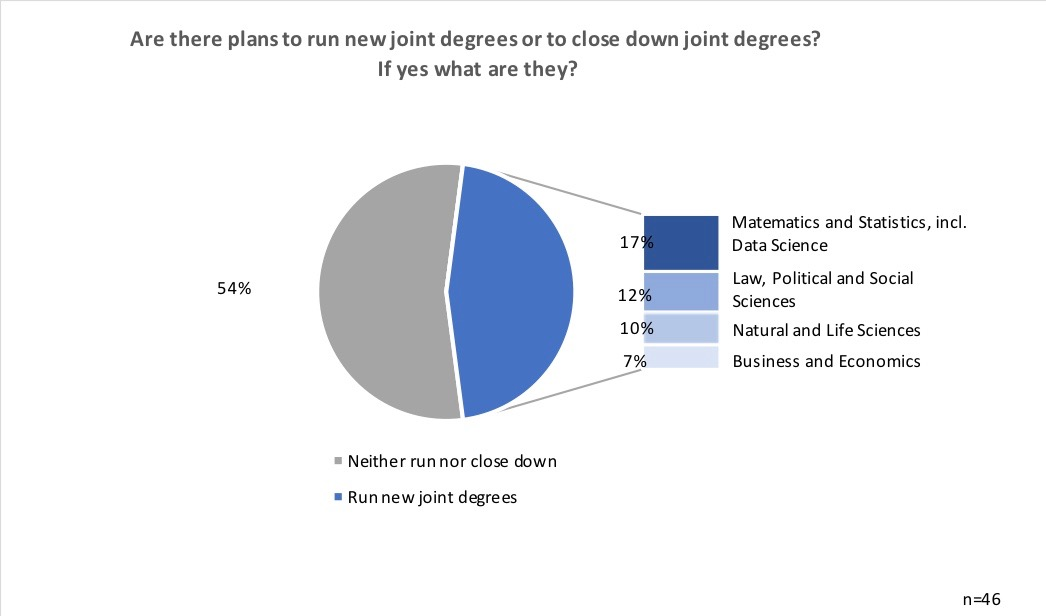
\includegraphics[width = \linewidth]{charts/2b.jpg}

In general, the situation is  quite stable for those universities that are currently offering joint degrees. Most of the universities not already offering joint degree show a significative interest in running new joint degrees. The most popular joint degrees to be run in the future are in the subject of Mathematics and Statistics for which at least eight universities have shown interest (IT University of Copenhagen, University of Edinburgh, University of Oviedo, Aalborg University, Paderborn, University of Malaga, University of Southern Denmark, Humboldt-Universität zu Berlin), followed by the subject of 
Natural and Life Sciences (University of Bern, University of Stuttgart, University of Lugano, Humboldt-Universität zu Berlin) and 
Law, social and political sciences (RWTH Aachen, Eötvös Loránd University, University of Edinburgh, University of Stuttgart, Paderborn) and finally the area of  Business and Economics (University of Edinburgh, University of Bari "Aldo Moro", Tilburg University). 

\section{2.C. Who teaches the Informatics component of non-Informatics degrees? For example, is programming taught to Physicists by members of the Physics department, of the Informatics department or is there a servicing organisation within your university that teaches Physics students to code (or some other mechanism)? }

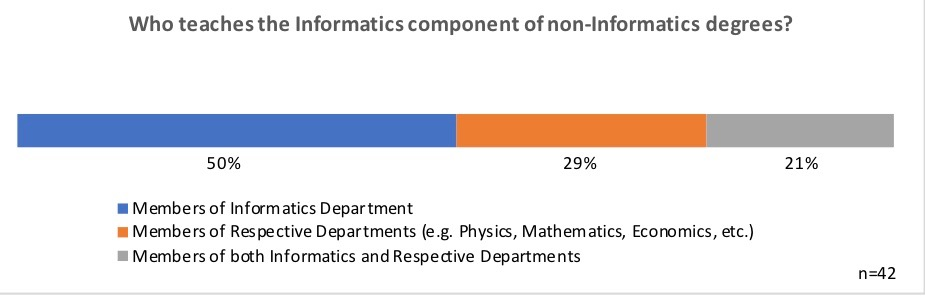
\includegraphics[width = \linewidth]{charts/2c.jpg}

The results of the survey indicates that half of the universities (50\%) give the responsability of teaching informatics subjects fo non-informatics degrees to members of the Informatics department. And additional 21\% of the universities the responsability of teaching Informatics is shared amog the Informatics department and other departments involved in the joint degree; some of the universities specify that only the general/basic subjects related to the Informatics of non-Informatics degrees are taught by Informatics department (for example programming) but when the subject is related to any particular contents of the degree and the informatics, then the subject is taught by the teachers with profile related with the specific degree. For example, the Bioinformatics of the Biotechnology degree is taught by Chemists. In other universities, informatics component of non-informatics degree programmes is sometimes taught by the informatics department, especially the more advanced levels. Some of the informatics departments have not enough human resources to acquire teaching responsabilities  for non-Informatics degrees . A significative percentage of the unversities consulted (29\%) recognize that informatics components of joint degrees are taught by other departments such as Physics, Mathematics, Economics, etc., depending on the subject of the joint degree.

\section{2.D. If Informatics is taught by people not located in an Informatics department are they Computer Scientists by training or research?}

A very low percentage of the answers (27\%) corresponds to universities where the informatics is always taught by teachers located at an informatics department. Nevertheless, an additional 22\% of the answers specify that the informatics is taught by Computer Scientists. Most of the universities participant in the survey recognize that persons who teach informatics for students of non-informatics degree does not have a background in Computer Science (51\%). Usually, when the Informatics subjects are  taught by non Computer Scientists, the teachers have a background formation in the same degree the students are following; e.g. electrical engineers at the Electrical Engeneering Schools, Economics/Management people at the Business School, Physists or Engineers at Robotics or Industrial engineering degrees. Additionally, in some universities the  basic informatics courses  are taught by non Computer Scientists.   





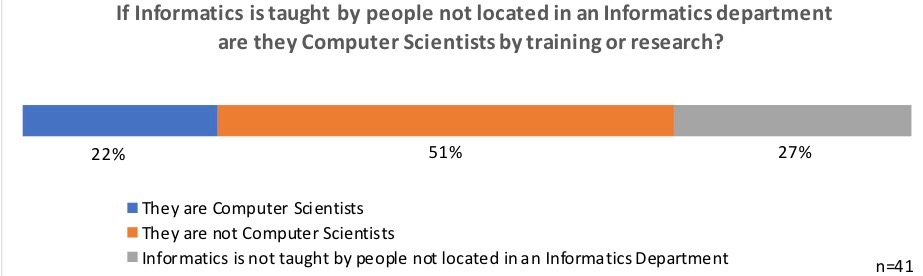
\includegraphics[width = \linewidth]{charts/2d.jpg}

\section{2.E. Please comment on any advantages or disadvantages you perceive of your university’s arrangements.}

The casuistry of the answers is really broad. For some universities there exits a clear discipline-responsibility (e.g. Paderborn) but in others there is no clear regulations about the department teaching informatics in non-informatics programmes (e.g. RWTH Aachen); lacks of human resources prevent the informatics departments to be in charge of teaching informatics subjects in non-informatics degree programmes (e.g. Utrecht University, Università Roma Tre, University of Bari "Aldo Moro",  Tilburg University)
